The \texttt{\pkglnk{model}} package contains the \texttt{\lnk{ExecutionEngine}}
class, which is used to reduce \texttt{\hyperref[type:edu.kit.wavelength.client.model.term.LambdaTerm]{LambdaTerm}}s.
It is initialized with an input string, as well as the reduction
order (see \texttt{\pkglnk{model.reduction}}), output size (see \texttt{\pkglnk{model.output}})
and included libraries (see \texttt{\pkglnk{model.library}}) and can then be used to
interactively operate on the lambda term, by stepping forward (that is, $\beta$-reducing according to 
the reduction order or reducing a provided redex in the current term) and backward (reverting to the 
previous term that was displayed).

The \texttt{\lnk{ExecutionEngine}} is fully synchronous and does not have a notion
of "fully" reducing a term.

\begin{figure}[H]
	\centering
	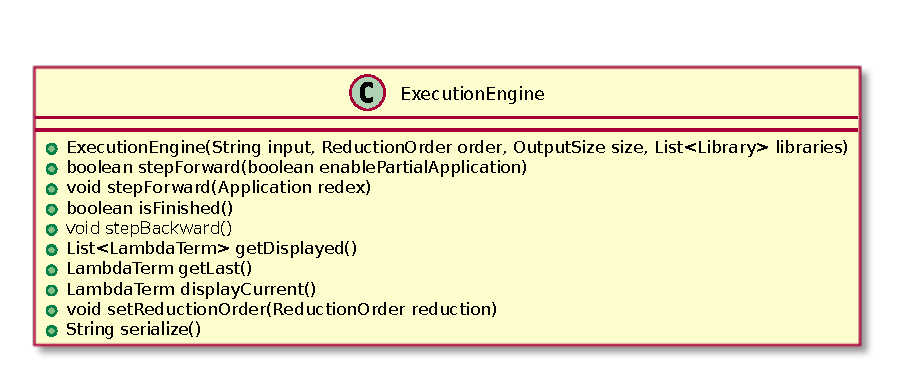
\includegraphics[width=\textwidth]{packageDiagrams/modelPackage}
\end{figure}
